%!TEX root = ../../../memoria.tex
\section{\shippingEF}\label{chapter:solucionimplementada:section:shipping}

	El proceso consiste en 6 pasos que deben cumplirse en orden estricto.

	En la parte superior de esta vista( \refFigura{figure:shipping:global_status}), se puede ver en todo momento el estado actual del \workflowCPT del proceso \shippingEF.

	\begin{figure}[H]
		\centering
		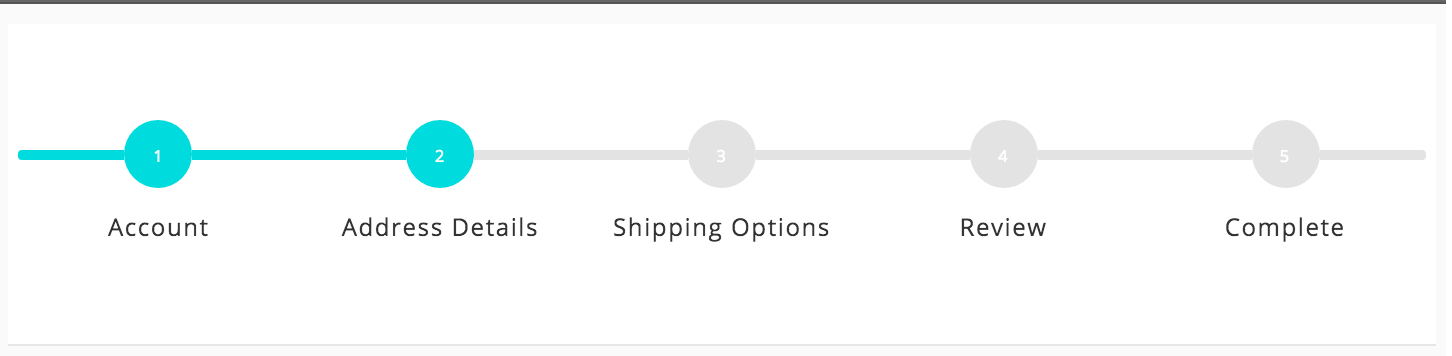
\includegraphics[width=0.7\textwidth]{figuras/shipping/global_status.png}
		\caption{Estado actual del \workflowCPT del \shippingEF. En este caso se encuentra en la selección de la dirección.}
		\label{figure:shipping:global_status}
	\end{figure}

	Adicionalmente a eso, la vista de \shippingEF muestra en detalle todos los pasos (\refFigura{figure:shipping:steps}). Cada uno de estos pasos se define como:

	\begin{description}
		\item[Account] \hfill \\
			Corresponde al proceso de autenticarse en la plataforma.
		\item[Address Details] \hfill \\
			Paso para la selección de una de las direcciones configuradas. Si no se tiene ningúna dirección agregada, el sistema muestra inmediatamente el formulario para la creación de una nueva dirección (\refFigura{figure:shipping:form_address}).
		\item[Shipping Options] \hfill \\
			Permite seleccionar uno de los métodos de envío disponibles. Estos son configurados por el administrador 
		\item[Review] \hfill \\
			Muestra un resumen de la información agregada al carro de compra. 
		\item[Complete] \hfill \\
			Paso de selección de método de pago.
	\end{description}


	\begin{figure}[H]
		\centering
		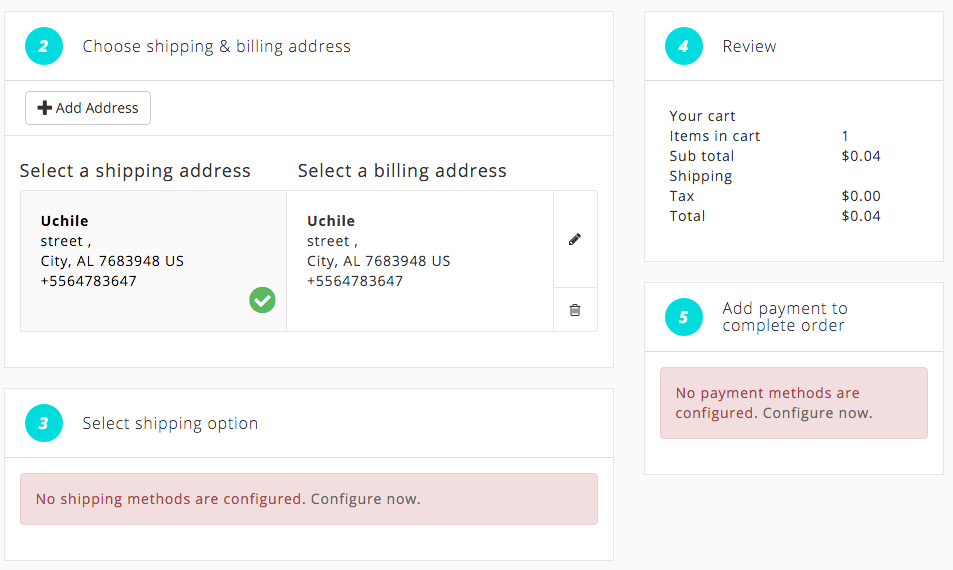
\includegraphics[width=0.8\textwidth]{figuras/shipping/steps.png}
		\caption{Detalle de todos los pasos del \workflowCPT \shippingEF.}
		\label{figure:shipping:steps}
	\end{figure}

	%TODO: modificar este texto despues
	En la \refFigura{figure:shipping:steps} se observa que los pasos 3 y 5 tienen un mensaje advirtiendo que no hay métodos de \shippingEF y métodos de pago configurados. Esta configuración debe ser realizada por el o los administradores de la tienda. Pero actualmente no están disponibles las interfaces para realizar estas acciones.

	\begin{figure}[H]
		\centering
		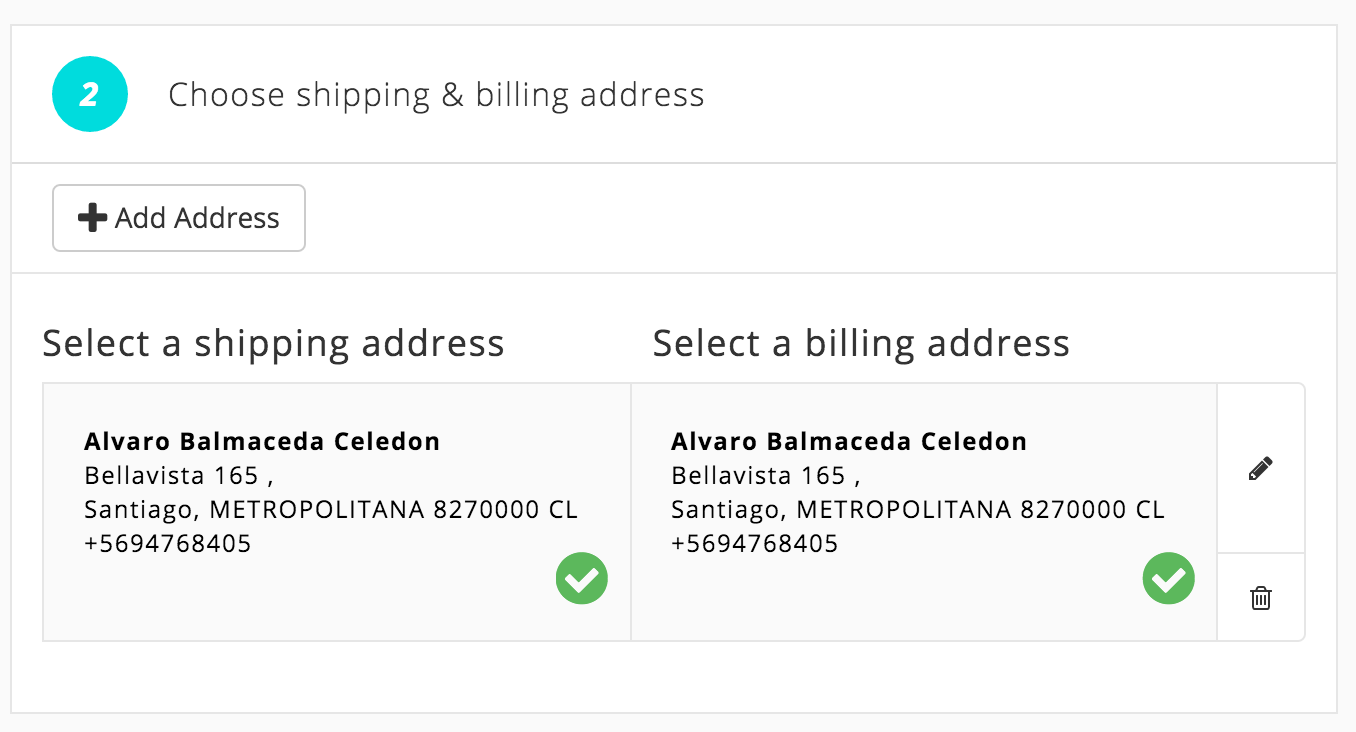
\includegraphics[width=0.8\textwidth]{figuras/shipping/step_address.png}
		\caption{Seleccionar dirección en proceso de \shippingEF.}
		\label{figure:shipping:step_address}
	\end{figure}

	\begin{figure}[H]
		\centering
		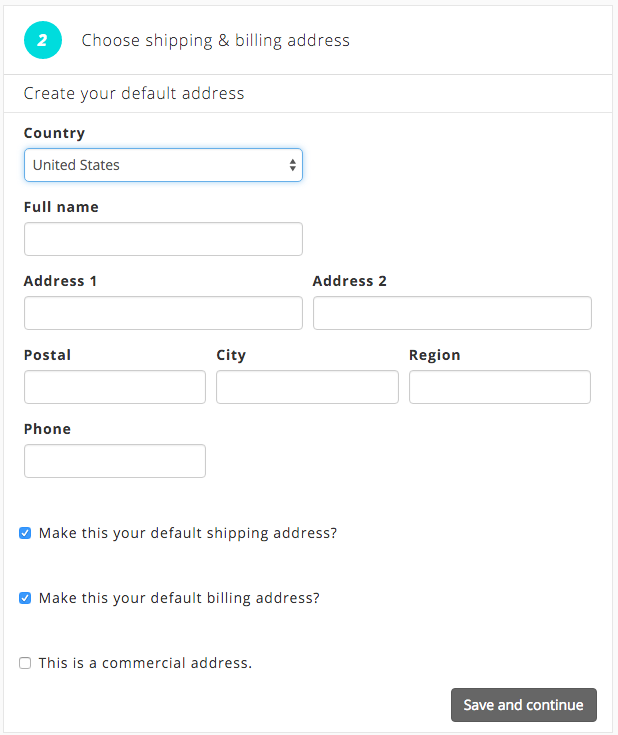
\includegraphics[width=0.6\textwidth]{figuras/shipping/form_address.png}
		\caption{Despliegue automático del formulario de direcciones cuando no se tienen ninguna dirección agregada.}
		\label{figure:shipping:form_address}
	\end{figure}


	En el caso de tener direcciones configuradas, pero se desee hacer el envío a una nueva dirección, es posible crearla apretando el botón \textit{Add Address} y un formulario se desplegará (\refFigura{figure:shipping:form_add_address}). Este formulario es equivalente al de la \refFigura{figure:shipping:form_address}, pero este incluye la opción de cancelar la creación de la dirección.

	\begin{figure}[H]
		\centering
		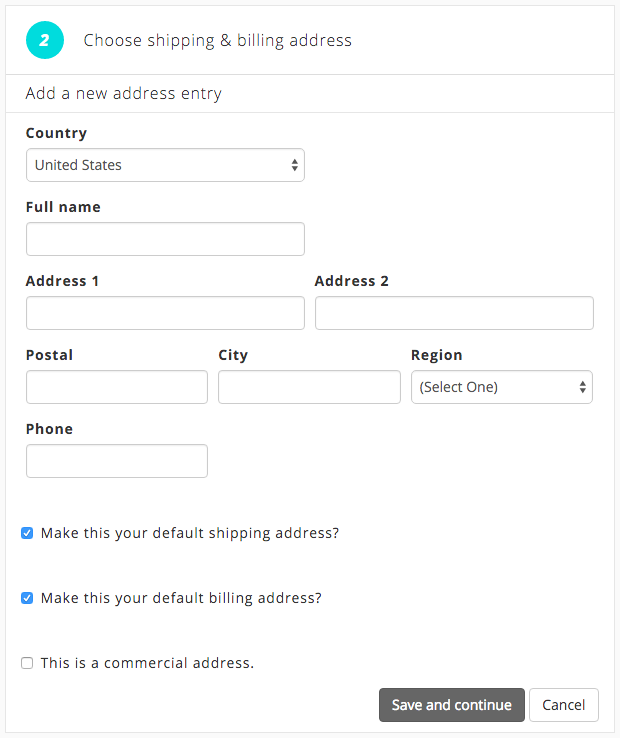
\includegraphics[width=0.6\textwidth]{figuras/shipping/form_add_address.png}
		\caption{Formulario de creación de una nueva dirección. Se diferencia del formulario de la \refFigura{figure:shipping:form_address} en que este incluye el botón Cancel.}
		\label{figure:shipping:form_add_address}
	\end{figure}